\section{DynamoDB}
    \subsection{Overview}
    A step for modeling data structure and figure out the data type are necessary before uploading data into the DynamoDB. After that, the table will be created and there will be some implementation for the table such as updating, deleting.The Information viewpoint will be use to design the table. Algorithm viewpoint will be use to implement different operation in database.    
    \subsection{Information viewpoint}
    The Information viewpoint will be use to modeling data structure (design the tables).
	\subsection{ Design Concern}
	The major concern will be modeling the data structure of NoSQL database in a clear way. It is very important because it will be easy to create tables if the modeling part is clear. Another concern will be how to convert data into schema in NoSQL database.In relational database, the ER-diagram is usually used to convert data into schema. In the key-value type of NoSQL database, the ER-diagram is not suitable to represent the table.The DynamoDB is much different with the SQL type database such as MySQL.In DynamoDB,we treat each rows of sample data as an individual item and each columns will be the attributes for the item.When we load the data into table, we are actually load the items into the table in DynamoDB.The figure \ref{fig:1} shows the example for this.

\begin{figure}[H]
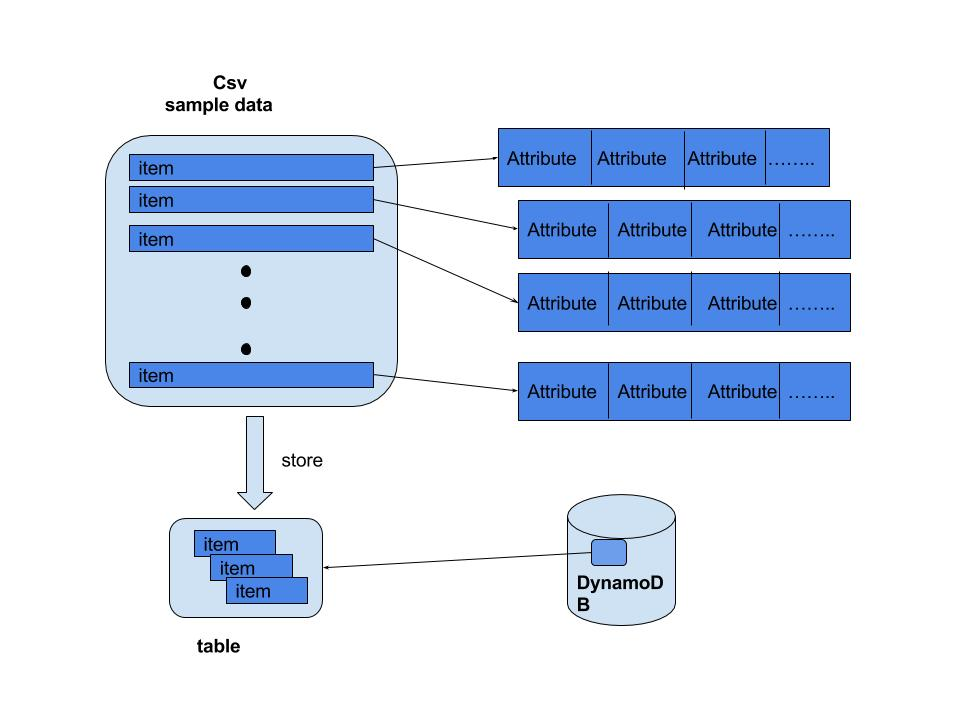
\includegraphics[width=15cm, height=12cm]{11.jpg}
\centering
\caption{\label{fig:1}sample csv data in DynamoDB table}
\end{figure}
 
	\noindent Based on the sample data, there will be three tables in the DynamoDB. The first table is called DataForcapstone1 which contains almost all the attributes except MAC address and ONID. Instead, there will be two linked tables which contains the MAC address and ONID. Each table will have unique keys and PINs, where the PINs are actually a hash of the ONID.By designing like this, the data analyst could give access control to different users for accessing the different tables. For example, a normal user might only have access to the main table, not the linked table.The figure \ref{fig:3} shows the process of this.

\begin{figure}[H]
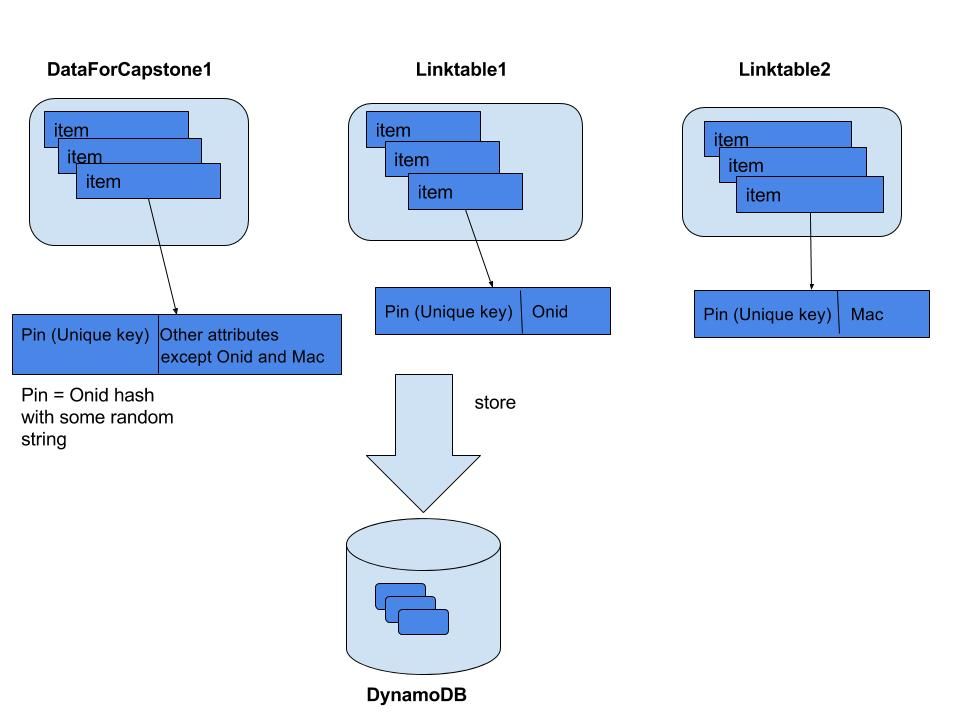
\includegraphics[width=15cm, height=8cm]{7.jpg}
\centering
\caption{\label{fig:3}sample csv data in DynamoDB table}
\end{figure}
	
    \noindent The workflow of loading new data into DynamoDB will start at S3. At first, the New record will be stored into S3. After that, we will check whether the ONID or MAC is new. If it is not new, we will replace the Pin with ONID or MAC address in the new record and store back to the S3.If the ONID or MAC is new, we will generate Pins base on hash the ONID.Then, we will load the new PINs, ONID and MAC into DynamoDB Identity table. This table will not be accessible for the users. After that, we will load the anonymized record into DynamoDB. The figure \ref{fig:5} shows the process of this.
    
\begin{figure}[H]
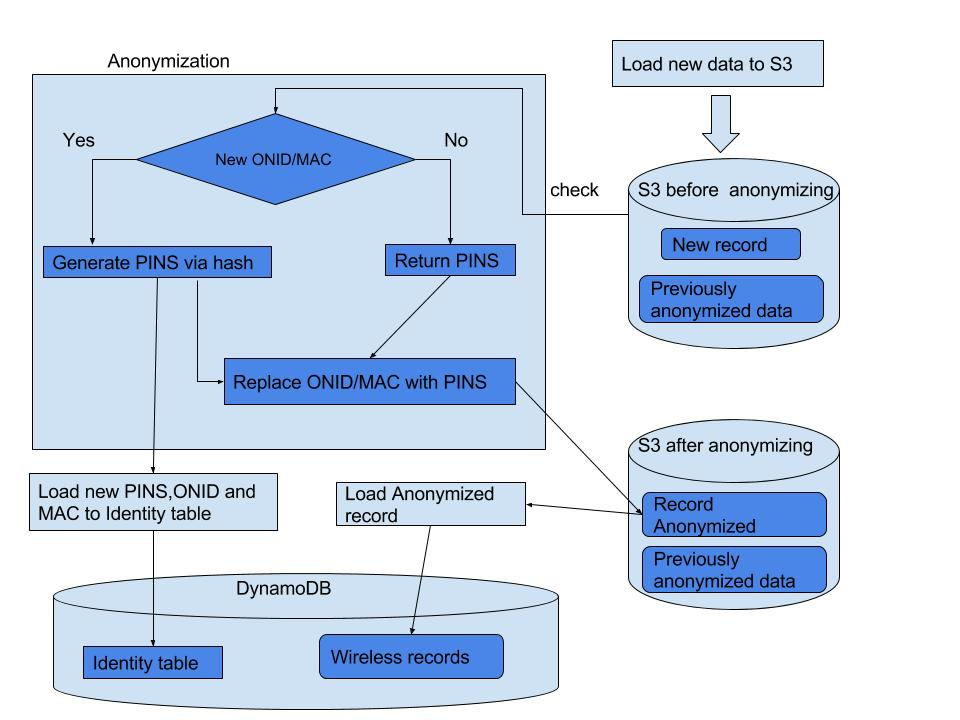
\includegraphics[width=15cm, height=9cm]{8.jpg}
\centering
\caption{\label{fig:5} workflow for loading new data }
\end{figure}
 

    \subsection{Algorithm viewpoint}
    Algorithm viewpoint will be use to implement different operation such as create table, upload data, update table, delete table, list table, query table and scan table.
    \subsection{Design concerns}
    The concern for this part will be how to design the algorithm for operations. Fortunately, the Amazon provides basic APIs for the operations. So we can adapt it from the Amazon document API. 
    \subsection{Boto 3}
    Boto 3 is actually the AWS SDK for Python. It allows the Python developer to write program that make use of the services on AWS such as EC2. In our project, We could use it to do different implementations for the table.For instance, if we need to update some items in the table, we could use the APIs in AWS Python SDK to do the updating.For this project we use it to creating table, uploading data and other implementations.
	\subsection{APIs for operation}
 	 	\subsubsection{Create Tables}
    	We will use the Boto 3 for creating tables. The Amazon provides the Python API for creating tables.These API will help us to create the database schema that we need.The API will first create a DynamoDB class. After that it declares a table request which contains the table name, key of table, the definitions of attributes.\\
Here is the API\cite{w1} :
\begin{lstlisting}[language=python, caption=API for create tables]
import boto3
dynamodb = boto3.resource('dynamodb')
table = dynamodb.create_table( //create tables
    TableName=' ',
    KeySchema=[
        {
            'AttributeName': 'username',
            'KeyType': 'HASH'
        },
    ],
    AttributeDefinitions=[
        {
            'AttributeName': 'username',
            'AttributeType': 'S'
        },
    ],
\end{lstlisting}
    	\subsubsection{Create an new item}
    	We will use the Boto 3 for creating an new item in schema. The Amazon provides Python API for  creating an new item.We will use these API to creating an new item in schema. The API will first select the DynamoDB table.After that it declares a new item which contains the primary key and the attributes for creating.\\
Here is the API\cite{w1}:
\begin{lstlisting}[language=Python, caption=API for creating an new item]
table = dynamodb.Table('tablename')
table.put_item(
   	Item={
        'Username': ' ',
        'Attribute1': '',
        'Attribute2': '',
        'Attribute3': ,
        'Attribute4': ' ',
    }
}
\end{lstlisting}
    \subsubsection{Update Table}
    We will use the Boto 3 for updating table. The Amazon provides Python API for updating table.We will use these API to update the data in the table that we create.The API will first select the DynamoDB table. After that it select the item which needs to update and update the information.\\
Here is the API\cite{w1}:
\begin{lstlisting}[language=Python, caption=API for updating table]
table = dynamodb.Table('tablename')
table.update_item(
    Key={
        'username': '',
    },
    UpdateExpression='SET age = :val1',
    ExpressionAttributeValues={
        ':val1': 26
    }
)
\end{lstlisting}
    \subsubsection{Delete Item}
    We will use the Boto 3 for deleting item. The Amazon provides Python API for deleting items. We will use these API to deleting Item.The API will first select the DynamoDB table. After that, it deletes the item which needs to delete.\\
Here is the API\cite{w1}:
\begin{lstlisting}[language=Python, caption=API for delete data]
table = dynamodb.Table('tablename')
table.delete_item(
    Key={
        'username': 'keyname',
    }
}
\end{lstlisting}
    \subsubsection{Query table}
    We will use the Boto 3 for query the table. The Amazon provides Python API for querying the table.We will use these API to query the table that we create. The API will first select the DynamoDB table.After that, it will use the query to retrieving the data.\\
Here is the API\cite{w1}:
\begin{lstlisting}[language=Python, caption=API for query table]
table = dynamodb.Table('tablename')
response = table.query(
	KeyConditionExpression=Key('username').eq('')
)
items = response['Items']
print(items)
}
\end{lstlisting}
    \subsubsection{Scan Table}
    We will use the Boto 3 for scan the table.The Amazon provides  Python API for scan the table.We will use these API to scan the table in order to read the data which store in the table. The API will first select the DynamoDB table.After that, it will use the scan to scan the data.\\
    Here is the API for Scan Table\cite{w1}:
\begin{lstlisting}[language=Python, caption=API for scan table]
table = dynamodb.Table('tablename')
response = table.scan(
    FilterExpression=Attr('Attributes').lt( )
)
items = response['Items']
print(items)
\end{lstlisting}

 \section{Quicksight}
    \subsection{Overview}
    The data store in the DynamoDB will be used to create an analyze and a visual on Amazon visualization tool called Quicksight. In this part, Information viewpoint will be used.
    \subsection{Information viewpoint}
    The information viewpoint can be used to achieve visualization part. Basically, we will use the Quicksight as the visualization tool to represent the analyzing result.
    \subsection{Design concern} 
    The major concern for this part will be how to generate a visual on the Quicksight. Fortunately, the Amazon provides tutorial on the Quicksight document. Therefore, we can a follow the instruction step by step from the document.    
    \subsection{Step for creating a visual}
    Base on the Quicksight document, there will be several general step for creating a visual. The first step is to create a data source in your database. These data source are very important for Quicksight because it will require these data source for creating data set and do the analyzing. After that, the Quicksight needs to connect with the data source. In this step, if the database is on the Amazon web services the data source will be easily to connect. However, if the data source is not on the Amazon web services it requires port, database access information to connect the data source in database. The detail information is on the Amazon Quicksight document. The next step is to create the data set according to data source and do an analyzing. The last step is to create a visual according to the data set. There are different types of visual on the Quicksight and we can choose one to generate the suitable graph for the analyzing result.\cite{w2}For our project, the QuickSight will get the data source and create the data set from S3 or Local PC.\\
    The figure \ref{fig:2} shows the general process:
    \begin{figure}[H]
    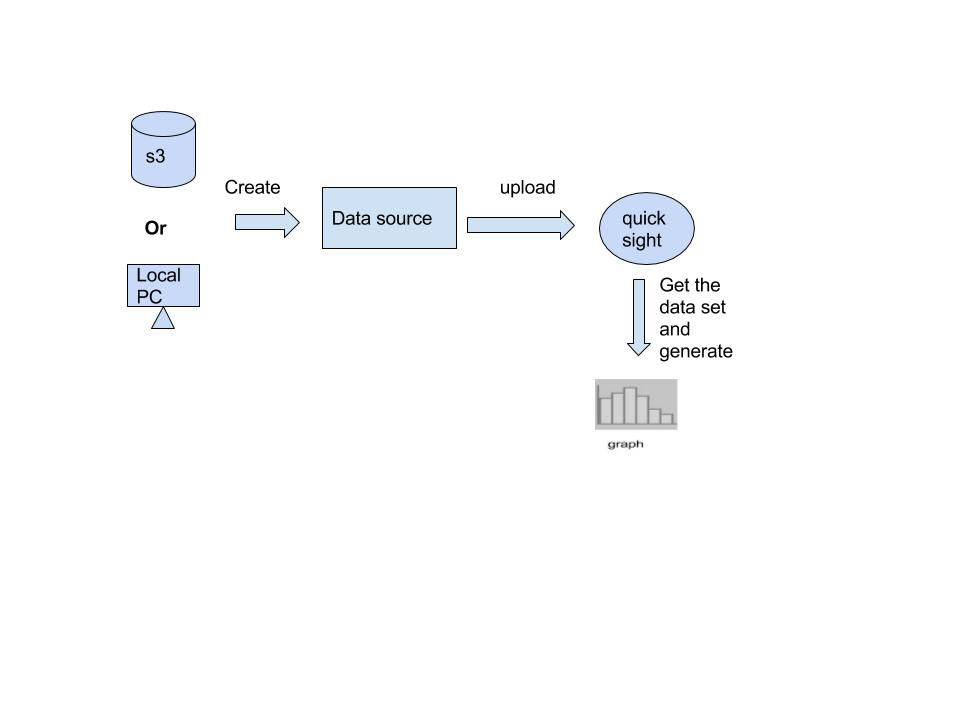
\includegraphics[width=16cm, height=8cm]{6.jpg}
    \centering
    \caption{\label{fig:2}General process}
    \end{figure}

